%%%%%%%%%%%%%%%%%%%%%%%%%%%%%%%%%%%%%%%%%
% Beamer Presentation
% LaTeX Template
% Version 1.0 (10/11/12)
%
% This template has been downloaded from:
% http://www.LaTeXTemplates.com
%
% License:
% CC BY-NC-SA 3.0 (http://creativecommons.org/licenses/by-nc-sa/3.0/)
%
%%%%%%%%%%%%%%%%%%%%%%%%%%%%%%%%%%%%%%%%%

%----------------------------------------------------------------------------------------
%	PACKAGES AND THEMES
%----------------------------------------------------------------------------------------

\documentclass{beamer}

\mode<presentation> {

% The Beamer class comes with a number of default slide themes
% which change the colors and layouts of slides. Below this is a list
% of all the themes, uncomment each in turn to see what they look like.

%\usetheme{default}
%\usetheme{AnnArbor}
%\usetheme{Antibes}
%\usetheme{Bergen}
%\usetheme{Berkeley}
%\usetheme{Berlin}
%\usetheme{Boadilla}
%\usetheme{CambridgeUS}
%\usetheme{Copenhagen}
%\usetheme{Darmstadt}
%\usetheme{Dresden}
%\usetheme{Frankfurt}
%\usetheme{Goettingen}
%\usetheme{Hannover}
%\usetheme{Ilmenau}
%\usetheme{JuanLesPins}
%\usetheme{Luebeck}
\usetheme{Madrid}
%\usetheme{Malmoe}
%\usetheme{Marburg}
%\usetheme{Montpellier}
%\usetheme{PaloAlto}
%\usetheme{Pittsburgh}
%\usetheme{Rochester}
%\usetheme{Singapore}
%\usetheme{Szeged}
%\usetheme{Warsaw}

% As well as themes, the Beamer class has a number of color themes
% for any slide theme. Uncomment each of these in turn to see how it
% changes the colors of your current slide theme.

%\usecolortheme{albatross}
%\usecolortheme{beaver}
%\usecolortheme{beetle}
%\usecolortheme{crane}
%\usecolortheme{dolphin}
%\usecolortheme{dove}
%\usecolortheme{fly}
%\usecolortheme{lily}
%\usecolortheme{orchid}
%\usecolortheme{rose}
%\usecolortheme{seagull}
\usecolortheme{seahorse}
%\usecolortheme{whale}
%\usecolortheme{wolverine}

\setbeamertemplate{footline} % To remove the footer line in all slides uncomment this line
%\setbeamertemplate{footline}[page number] % To replace the footer line in all slides with a simple slide count uncomment this line

\setbeamertemplate{navigation symbols}{} % To remove the navigation symbols from the bottom of all slides uncomment this line
}

\usepackage{graphicx} % Allows including images
\usepackage{ulem} % Allows including images
\usepackage{xcolor} % Allows including images

\let\oldfootnotesize\footnotesize
\renewcommand*{\footnotesize}{\oldfootnotesize\tiny}

\newcommand\rem{\bgroup\markoverwith{\textcolor{red}{\rule[.3ex]{2pt}{1.5pt}}}\ULon}

\title{Fully Polynomial Parameterized Algorithms\\For the \texorpdfstring{$T$}{T}-Path Packing Problem} % The short title appears at the bottom of every slide, the full title is only on the title page

\author{Narek Bojikian} % Your name
\institute[Hu-Berlin]
{
	Humboldt University of Berlin
}
\date{12.12.2019} % Date, can be changed to a custom date

\begin{document}

\begin{frame}
\titlepage % Print the title page as the first slide
\end{frame}
%\begin{frame}[t]{Introduction}
%	\vspace{10px}
%	\begin{minipage}[t]{0.5\linewidth}
%		\begin{itemize}[<+->]
%			\item $T$-path packing.
%			\item Odd $T$-path packing.
%			\item $S-T$-path packing.
%			\item[--] Goal: Find maximum set of each.
%			\item Maximum Matching - $\nu(G)$.
%		\end{itemize}
%	\end{minipage}\hfill
%	\begin{minipage}{0.5\linewidth}
%		\centering
%		
\includegraphics{figures/graph.eps}
%	\end{minipage}
%\end{frame}

\begin{frame}[t]{Introduction}
	\begin{columns}
		\begin{column}{.5\textwidth}
			\begin{itemize}[<+->]
				\uncover<1->{\item $T$-path packing.}
				\uncover<3->{\item Odd $T$-path packing.}
				\uncover<5->{\item $S-T$-path packing.}
				\uncover<7->{\item[--] Goal: Find maximum set of each.}
				\uncover<8->{\item Maximum Matching - $\nu(G)$.}
			\end{itemize}
		\end{column}
		\begin{column}[c]{.5\textwidth}
			\centering
			\vspace{2cm}
			\only<1>{\makebox[\textwidth][c]{
\includegraphics{figures/t-graph.eps}}}
			\only<2>{\makebox[\textwidth][c]{
\includegraphics{figures/t-path.eps}}}
			\only<3>{\makebox[\textwidth][c]{
\includegraphics{figures/t-graph.eps}}}
			\only<4>{\makebox[\textwidth][c]{
\includegraphics{figures/odd-t-path.eps}}}
			\only<5>{\makebox[\textwidth][c]{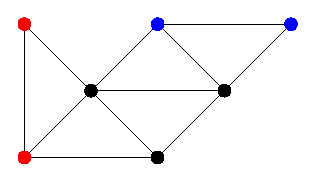
\includegraphics{figures/st-graph.eps}}}
			\only<6-7>{\makebox[\textwidth][c]{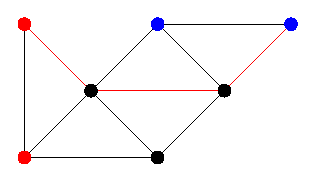
\includegraphics{figures/st-path.eps}}}
			\only<8>{\makebox[\textwidth][c]{
\includegraphics{figures/graph.eps}}}
			\only<9>{\makebox[\textwidth][c]{
\includegraphics{figures/matching.eps}}}
		\end{column}
	\end{columns}
\end{frame}

\begin{frame}[t]{Reduction - $T$-Path Packing to Matching}
	\begin{minipage}[t][.4\textheight][t]{\linewidth}
		An instance of the $T$-path packing problem.
	\end{minipage}
	\hfill
	\begin{minipage}[t][.4\textheight][t]{\linewidth}
		The corresponding maximum matching instance.
	\end{minipage}
\end{frame}

\begin{frame}[t]{Reductions presented in the thesis}
	\begin{minipage}[t][.3\textheight][t]{\linewidth}
		\begin{minipage}[t][\textheight][t]{.45\linewidth}

			$T$-path packing first reduction.
			
		\end{minipage}
		\hfill
		\vline
		\hfill
		\begin{minipage}[t][\textheight][t]{.45\linewidth}
			$T$-path packing second reduction.
		\end{minipage}
	\end{minipage}
		\vfill
		\hrule
		\vfill
	\begin{minipage}[t][.3\textheight][t]{\linewidth}
		\begin{minipage}[t][\textheight][t]{.45\linewidth}
			Odd $T$-path packing second reduction.
		\end{minipage}
		\hfill
		\hfill
		\begin{minipage}[t][\textheight][t]{.45\linewidth}
			$S-T$-path packing second reduction.
		\end{minipage}
	\end{minipage}

\end{frame}

\begin{frame}{Methods and results - Preserving properties}
[Do two frames per method one example and one list of params]

[todo: check results]

[todo: add running times?]
\end{frame}
\begin{frame}[t]{Methods and results - Preserving properties}
\vspace{.5cm}
	\begin{itemize}
		\item $T$-path packing (using the second reduction):
		\begin{itemize}
			\item[--] Tree-depth.
			\item[--] Tree-width.\\ \hspace{.5cm} The value at most doubles.
			\item[--] Modular-width.
			\item[--] Independence number.
			\item[--] Neighborhood diversity number.
			\item[--] $s$-plexes.\\ \hspace{.5cm} The value does not change.
			\item[--] Strongly chordal graphs.
			\item[--] Interval- Circular-arc- and co-Comparability- graphs.\\
				\hspace{.5cm} The classes are closed under this reduction.
		\end{itemize}
	\end{itemize}
\end{frame}

\begin{frame}[t]{Methods and results - Preserving properties}
\vspace{.5cm}
	\begin{itemize}
		\item Odd $T$-path packing:
			\begin{itemize}
				\item[--] Neighborhood diversity number\\
					\hspace{.5cm} - bounded Replaceablity.
			\end{itemize}
		\item Odd $T$-path packing and $S-T$-path packing:
			\begin{itemize}
				\item[--] Tree-depth, tree-width and modular-width\\
					\hspace{.5cm} - as in $T$-path packing.
				\item[--] \rem{Independence number - does not change}
			\end{itemize}
	\end{itemize}
\end{frame}

\begin{frame}[t]{Methods and results - Distance to triviality}
\vspace{.5cm}
\begin{itemize}
	\uncover<1->{\item Vertex-deletion distance to a class - $d_{\mathcal{\mathcal{C}}}(G)$.}


	\uncover<2->{\item The reductions preserve the distance to triviality.\\}
		\uncover<3->{Given a graph $G$, a class $\mathcal{C}$ and any of the reductions $f$ such that\\
		\hspace{.5cm} $\mathcal{C}$ is closed under $f$ and $d_{\mathcal{C}}(G) \leq k$, then
	\hspace{.5cm} \textcolor{blue}{$d_{\mathcal{C}}(f(G)) \leq 2k$}.}

	\uncover<4->{\item The reductions preserve the distance to parameters values.\\}
		\uncover<5->{Let $\rho_G$ be the value of the parameter in $G$. Consider the class $\mathcal{C}_n := \{G : \rho_G \leq n\}$. For a reduction $f$, such that $f(C_n) \subseteq C_{g(n)}$ for some computeable function $g$,\\
	\hspace{.5cm} we get \textcolor{blue}{$d_{\mathcal{C}_{g(n)}}(f(G)) \leq 2d_{C_n}(G)$}.}
	\end{itemize}
\end{frame}

\begin{frame}[t]{Methods and results - Distance to triviality}
\vspace{.5cm}
\begin{itemize}
	\uncover<1->{\item $T$-Path Packing.
		\begin{itemize}
			\item[--] Neighborhood diversity number.
			\item[--] $s$-plexes.
			\item[--] Independence number. [Again, only for this problem.]
		\end{itemize} }
	\uncover<2->{\item Odd $T$-Path Packing.\\
		Neighborhood diversity number.
		\begin{itemize}
			\uncover<3->{\item[--] The class of $\ell$-Replaceable graphs - $\mathcal{R}[\ell]$.}
			\uncover<4->{\item[--] or $m := |E(G)|$, $l, k \in \mathbb{N}$,  if $d_{\mathcal{R}[\ell]}(G) \leq k$,\\
				\hspace{.5cm} then $\nu(G)$ can be found in $O(\sqrt{k}\ell m)$
				\footnote{On adaptive algorithms for maximum matching, F.Hegerefeld and S.Kratsch, ICALP-2019.}.}
			\uncover<5->{\item[--] For $G'$ the graph resulting from $G$ when we apply the second reduction.\\
				If the Neighborhood diversity number of $G$ is at most $k$ then $G'$ is at most $2k$ replaceable.}
		\end{itemize}
	}
\end{itemize}
\end{frame}

\begin{frame}{Methods and results - Simplify, solve and augment}
\end{frame}
\begin{frame}[t]{Methods and results - Simplify, solve and augment}
\vspace{.5cm}
	\begin{itemize}
		\item Vertex Cover Number\\ \hspace{.5cm} - simplify to an independent set.
		\item Feedback Vertex Number\\ \hspace{.5cm} - simplify to a forest.
	\end{itemize}
	Designed a dynamic programming algorithm in trees.
\end{frame}

\end{document}
